% ================================== HEADER ====================================
\documentclass{article}           % Sets style/look of many things.
% \documentclass{report}          % part, chapters, front page etc.
\usepackage{exsheets}
\usepackage[utf8]{inputenc}       % Encoding of input files UTF-8
\usepackage[T1]{fontenc}
\usepackage[scaled]{beramono}     % Font
\usepackage{color}                % Color text
\usepackage{titlesec}             % Select alternative section titles
\usepackage{fancyvrb}
\usepackage{verbatim}             % Comment environment
\usepackage{listings}             % Format and render text/code etc.
\usepackage{minted}               % Much better syntax highlighting
\usepackage{float}                % Control of floating environment/figure
\usepackage{graphicx,  subfigure} % Better figures, graphics, units etc.
\usepackage{multicol}             % Multiple columns
\usepackage{amsmath}              % Math: Equation, split, align etc.
\usepackage{siunitx}              % SI units
\usepackage{mathtools}            % Different math tools to use with amsmath
\usepackage{amssymb}              % Math symbols
\usepackage[
    colorlinks,
    citecolor=black,              % I like links with standard black color
    filecolor=black,
    linkcolor=black,
    urlcolor=black
]{hyperref}                       % Links in TOC etc.
\usepackage[all]{hypcap}          % Better links to floating environment

\usepackage{tabto}
\newcommand\marginsymbol[1][0pt]{%
  \tabto*{0cm}\makebox[\dimexpr-1cm-#1\relax][r]{$\mathbb{P}$}\tabto*{\TabPrevPos}}

\renewcommand{\thesubsection}{\thesection.\alph{subsection}}
\title{\vspace{-2cm}INF3490/INF4490 Exercises - Week 3}
\author{Ole Herman Schumacher Elgesem, Magnus Olden, Stian Petlund}
\date{\today}

% Removing paragraph indents is sometimes useful:
\setlength\parindent{0pt}

% Make margins smaller to fit more figures, tables etc on page: (optional)
\addtolength{\oddsidemargin}{-1.0in}
\addtolength{\evensidemargin}{-1.0in}
\addtolength{\textwidth}{2.0in}
\addtolength{\topmargin}{-0.8in}
\addtolength{\textheight}{1.6in}
% ==============================================================================

% ================================= EXAMPLES ===================================
\begin{comment}

% TABLE (TABULAR):
\begin{table}[]
\centering
  \begin{tabular}{|l|c|c|c|}
    \hline
    Colors: & Red    & Green  & Blue \\ \hline
    Red     & Red    & Yellow & Purple \\ \hline
    Green   & Yellow & Green  & Cyan \\ \hline
    Blue    & Purple & Cyan   & Blue \\ \hline
  \end{tabular}
  \caption{Caption}
  \label{tab:my_label}
\end{table}

% FIGURE:
The plot in figure \ref{fig:unique_name} clearly shows something important.
\begin{figure}[H]
\begin{center}
\includegraphics[width=0.3\textwidth]{figs/silicon.png}
\caption{The caption explains the figure.}
\label{fig:unique_name}
\end{center}
\end{figure}

% EQUATION:
\begin{equation}
\frac{df}{dt} = \lim_{h \to 0}\frac{f(t+h)-f(t)}{h}
\end{equation}

% ALIGNED MATH:
\begin{align*}
    r      &= \sqrt{x^2 + y^2 + z^2} & x &= r\cos \theta \sin \phi \\
    \theta &= \tan^-1(\frac{y}{x})   & y &= r\sin \theta \sin \phi \\
    \phi   &= \cos^-1(\frac{z}{r})   & z &= r\cos \phi
\end{align*}

% CENTERED DISPLAY MODE MATH:
\[ V_{th} = 0.45V \]

% INLINE MATH:
We used a supply voltage of 1.2 volts; \(V_{dd} = 1.2\text{V}\).

% MATRIX:
\[
\begin{Bmatrix} % Curly brackets
v_1 \\
v_2
\end{Bmatrix}
= \begin{bmatrix} % Square brackets
Z_{11} & Z_{12} \\
Z_{21} & Z_{22}
\end{bmatrix}
\begin{Bmatrix}
i_1 \\
i_2
\end{Bmatrix}
\]

% COLORS:
\definecolor{orange}{RGB}{255,127,0}
{\color{red} Red text.} {\color{orange} Orange text.}

% SOURCE CODE:
\inputminted{Python}{src/hello.py}

% MULTIPLE COLUMNS:
\begin{multicols}{2}
Write text and add figures etc. Content will be automatically split. You can
put figures, tables and even other multicols. Multiple columns can reduce
wasted space in a document.
\end{multicols}

% FOOTNOTES:
A simple footnote\footnote{Additional information} or
footnotemark\footnotemark{} is more readable.
\footnotetext{Footnotes are usefule for definitions, clarifications,
background info, e-mail/website info etc.}

\end{comment}
% ==============================================================================

% ================================= DOCUMENT ===================================
\begin{document}
    \renewcommand\marginsymbol[1][0pt]{%
  \tabto*{0cm}\makebox[-1cm][c]{$\mathbb{P}$}\tabto*{\TabPrevPos}}

\maketitle
\(\mathbb{P}\) marks the programming exercises, we strongly recommend using
the python programming language for these. Exercises may be added/changed
after publishing.

\section{Pareto Optimality}
\begin{figure}[H]
  \centering
  \begin{minipage}[b]{0.45\textwidth}
    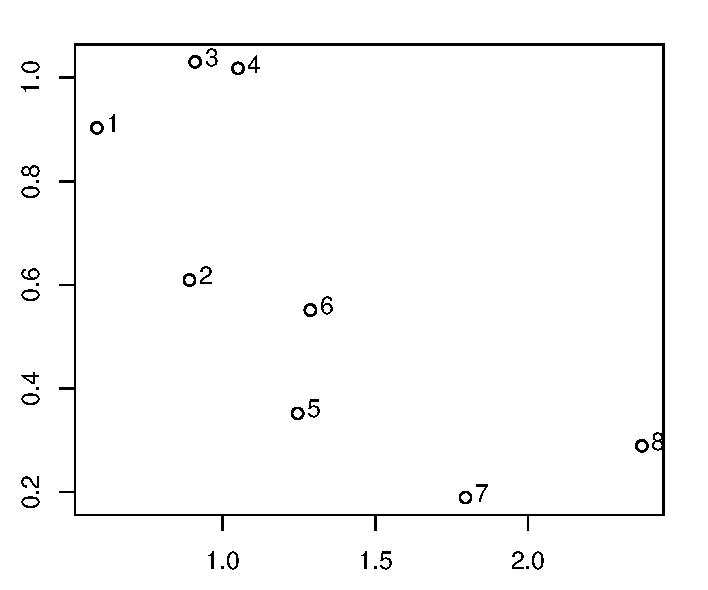
\includegraphics[width=\textwidth]{front_points_1.pdf}
    \caption{a}
  \end{minipage}
  \hfill
  \begin{minipage}[b]{0.45\textwidth}
    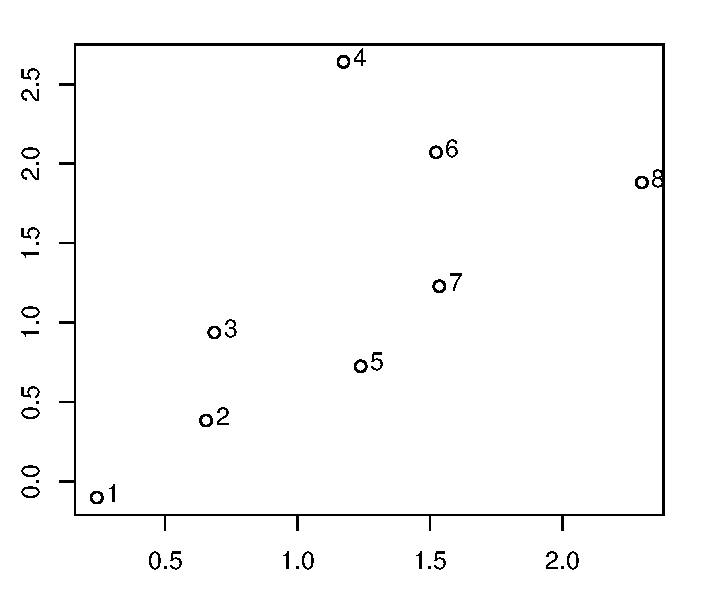
\includegraphics[width=\textwidth]{front_points_2.pdf}
    \caption{b}
  \end{minipage}
\end{figure}

For figure a and b above, find the Pareto optimal set when
\begin{itemize}
    \item Minimizing both \(f_1\) and \(f_2\)
    \item Minimizing \(f_1\), maximizing \(f_2\)
    \item Maximizing \(f_1\), minimizing \(f_2\)
    \item Maximizing both \(f_1\) and \(f_2\)
\end{itemize}
\section{Weighted sum}
In figures a and b, what would be the maximum point when using weighted sum:
\begin{itemize}
    \item \(w_1 = 1\),  \(w_2 = 1\)
    \item \(w_1 = -1\), \(w_2 = 1\)
\end{itemize}
\section{Hybrid Algorithm}
Why can hybrid algorithms make it harder to maintain diversity?
\section{Measuring algorithm performance}
Why is it usually better to use the number of fitness function evaluations as a
time measure, rather than the number of generations, or the amount of CPU
time spent?
\section*{Corrections and suggestions}
Corrections of grammar, language, notation or suggestions for improving these exercises are appreciated.
E-mail me at: \href{mailto:olehelg@uio.no}{\textbf{olehelg@uio.no}} or use
\href{https://github.com/olehermanse/INF3490-AI_Machine_Learning}{\textbf{GitHub}}
to submit an issue or create a pull request.
\end{document}
% ==============================================================================
